\subsection{SIR}

\begin{frame}
        \frametitle{Modèle SIR}

<<<<<<< HEAD
        \begin{center}
                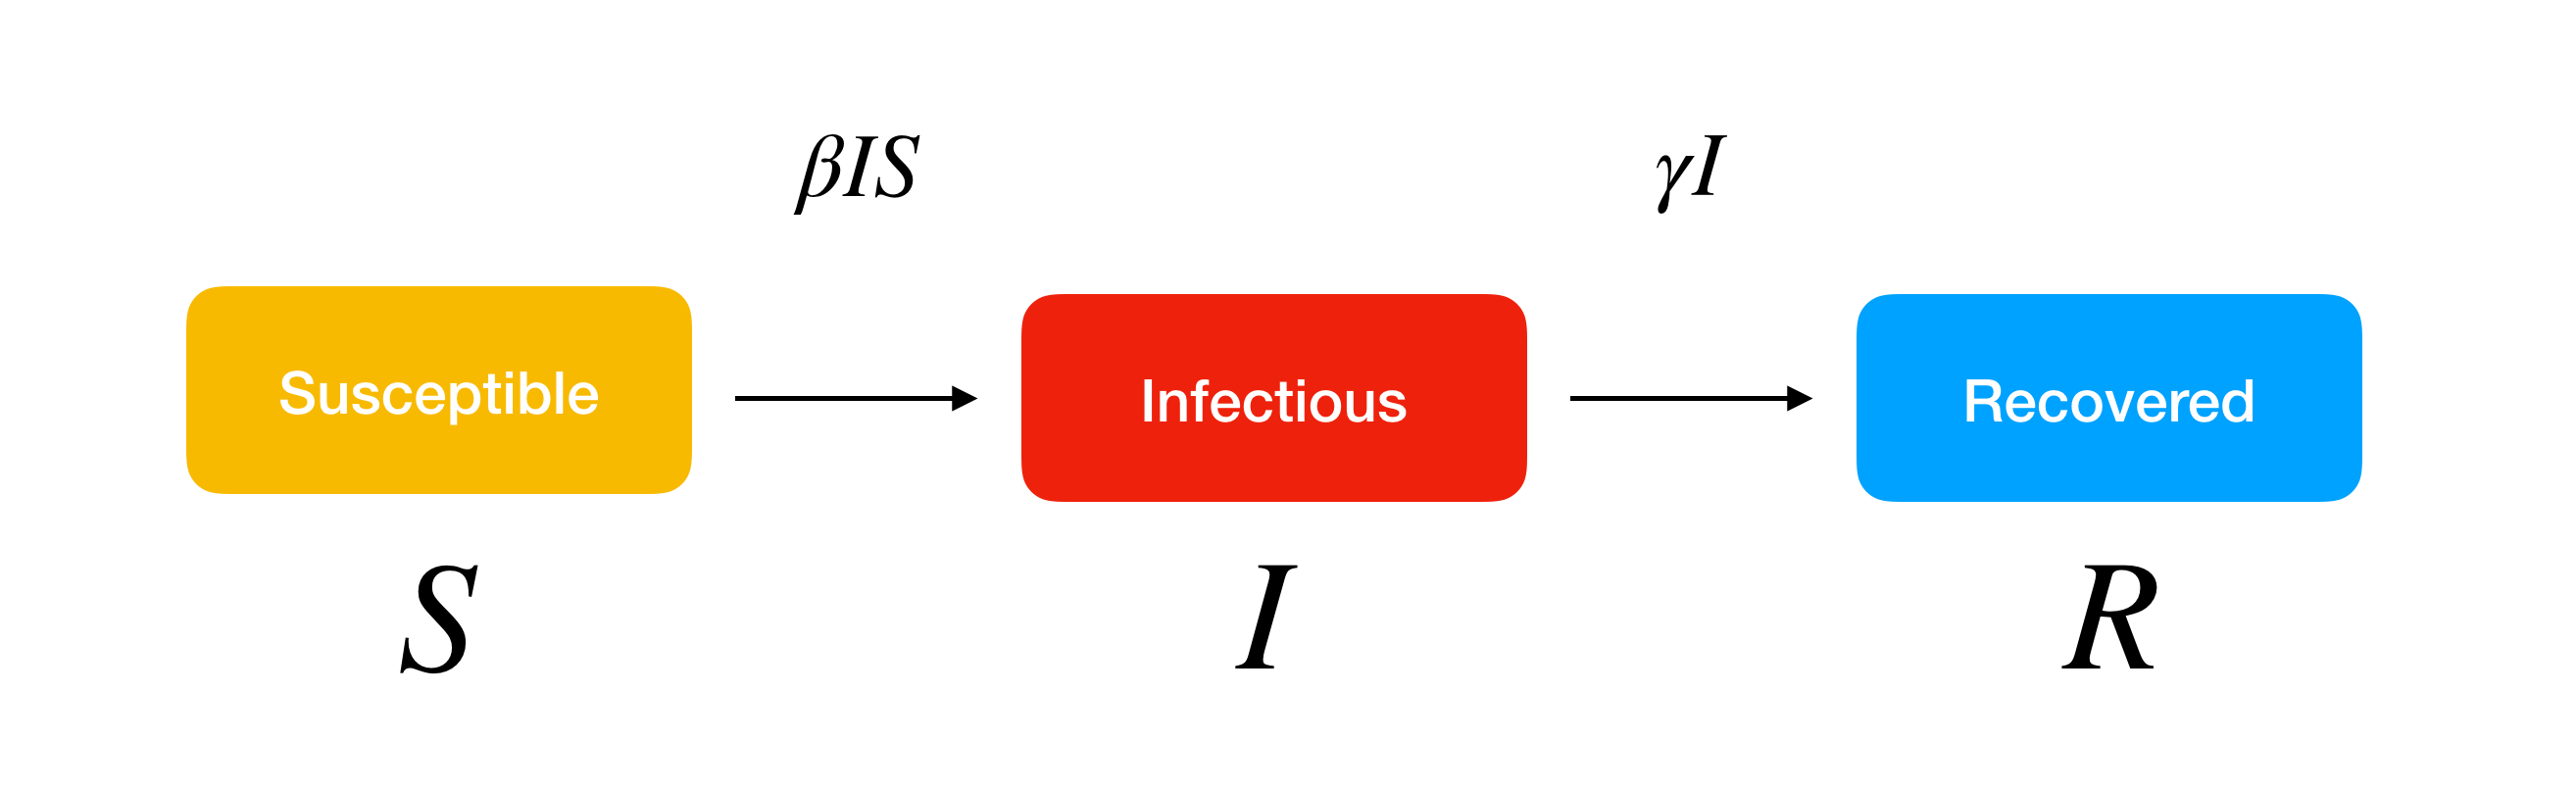
\includegraphics[width=0.75\textwidth]{sir_definition}
        \end{center}


        \begin{itemize}
                \item Susceptible - personnes saines qui n'ont pas encore contracté la maladie
                \item Infectés - les malades qui transmettent activement la maladie
                \item Rétablis - les personnes rétablies ou mortes, qui ne peuvent plus contracter la maladie.
        \end{itemize}

\end{frame}


\begin{frame}
        \frametitle{Modèle SIR}

        \begin{alertblock}{Équation}

                $$ \frac{dS}{dt} = -\frac{\beta SI}{N} \qquad \frac{dI}{dt} = \frac{\beta SI}{N} - \gamma I \qquad \frac{dR}{dt} = \gamma I $$

                \begin{itemize}
                        \item $N$ : taille totale de la population
                        \item $\beta$ : taux de contact
                        \item $\gamma$ : taux de guérison
                \end{itemize}

        \end{alertblock}
\end{frame}


\begin{frame}
        \frametitle{Modèle SIR}
        		\centering

		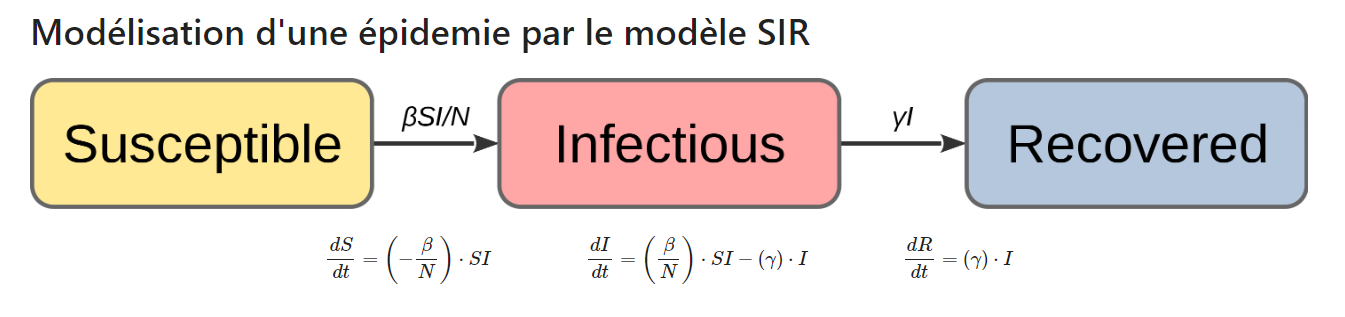
\includegraphics[width=1\linewidth]{SIRMODEL}
\end{frame}	
	 

\begin{frame}
        \frametitle{Modèle SIR}

		\centering

		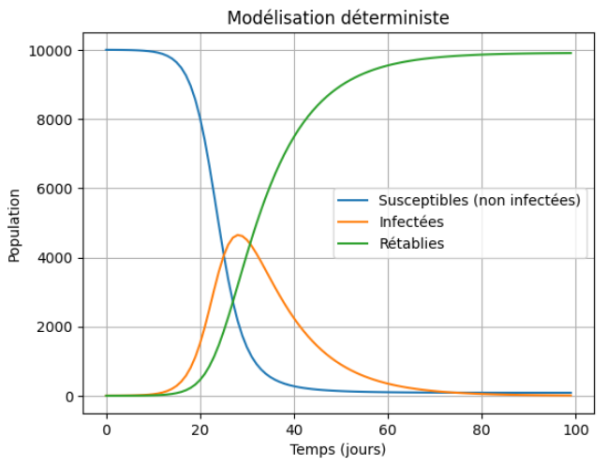
\includegraphics[width=0.45\linewidth, height=0.45\textheight, valign=c]{sir_deterministe}
		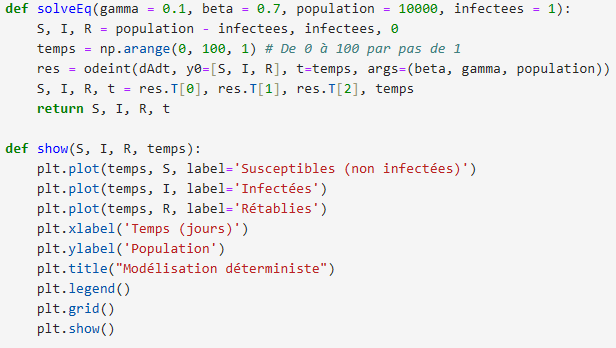
\includegraphics[width=0.5\linewidth, height=0.4\textheight, valign=c]{sir_deterministe_python}
		
        \begin{multicols}{2}
                \begin{itemize}
                        \item $\gamma = 0.1$
                        \item $\beta = 0.48$
                        \item $N = 10000$
                        \item $I_0 = 1$
                \end{itemize}
        \end{multicols}

\end{frame}


